\label{chapter:ModelExecution}
The steps in our model excution  workflow are:
\begin{enumerate}
    \item Run \mfus to create the new project output files (e.g.\ time-varying hydraulic head, drawdown etc).\label{step:modflow}
    \item Run \mut\ to post-process the \mfus\ simulation, which produces \tecplot\ output files for the various model domains (i.e.\ \gwf, \swf\ and/or \cln ) created during the simulation.\label{step:mut2}
    \item Run \tecplot\ and examine the \mfus\ output files.   \label{step:Tecplot2}
\end{enumerate}

\section{\mfus\ Simulation}
To run \mfus\ on the \texttt{1\_VSF\_Column} example, and assuming we have a command prompt open at the appropriate directory, we can type:
\begin{verbatim}
    usgs_1 modflow
\end{verbatim}
which obtains the prefix for the \mfus\ input files, in this case the default prefix {\sf modflow}.

 As \mfus\ processes the input file, output is written to the screen:

        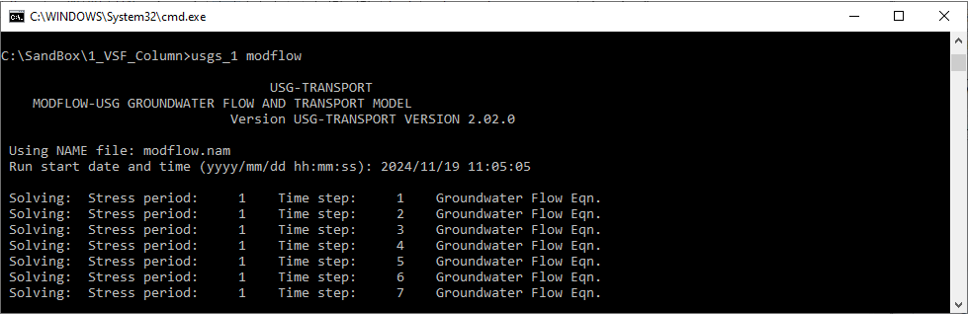
\includegraphics[width=\textwidth]{4_1_RunScreen}

 If execution is successful you will see the {\sf Normal termination of simulation} message:

        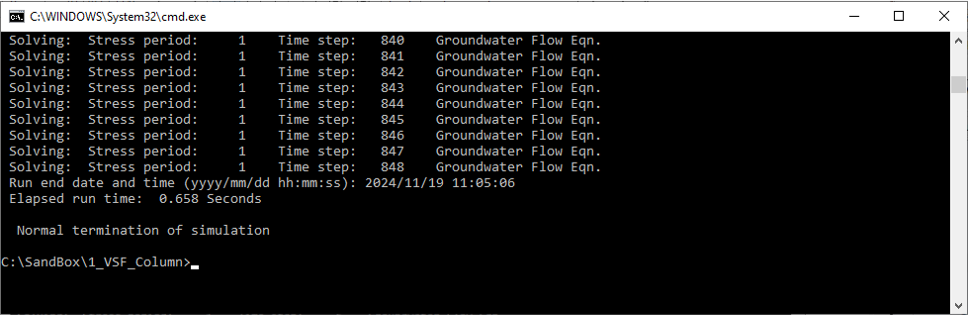
\includegraphics[width=\textwidth]{4_1_RunScreenExit}

 Every \mfus\ simulation generates a run-time
listing file, in this case called {\tt modflow.lst}, that consists of the input data for the simulation;
the solver and nonlinear outputs at user-requested detail; head
and drawdown solutions, if requested; mass-balance information; and time-step information for the simulation.  It also produces binary files of head, drawdown, saturation and cell-by-cell flows for each model domain.

To post-process the output produced by \mfus\ for the \texttt{1\_VSF\_Column} example, we would  run \mut\ using the input file \texttt{\_post.mut} by typing:
\begin{verbatim}
    mut _post
\end{verbatim}

If you open the file \texttt{\_post.mut} in a text editor you will see the first  line is a comment followed by one instruction and input:
\squish
\begin{verbatim}
    ! This example reads a modflow project and postprocesses it
    postprocess existing modflow model
        modflow
\end{verbatim}
As in the model build, \mut\ first creates a clean copy of the input file called \texttt{\_posto.input} by removing all comment lines.
 As it processes the input file, output is written to both the screen and to the file \texttt{\_posto.eco}.

\section{\mut\ Post-processing}
The instruction to post-process the \mfus\ model after execution is:

\ins{postprocess existing modflow model}
    {
        \squish
        \begin{enumerate}
        \item \str{Prefix}  The \mfus\ model prefix.
        \end{enumerate}
        Given \str{Prefix}, this instruction:
         \begin{itemize}
            \item  Reads head, drawdown and cell-by-cell flow binary output files for each output time and writes the results to the file {\tt \_posto.modflow.GWF.tecplot.dat}.
            \item scans the \mfus\ listing file, extracts volumetric budget data at each time step and writes the results to the file {\tt \_posto.modflow.VolumeBudget.tecplot.dat}.
         \end{itemize}
        \squish
    }

\section{Volumetric Water Budget Plots}
\index{Volumetric water budget}
Volumetric water budget data is useful for checking the fluid mass balance of the model run.  The example {\tt 4\_SWF\_RCH\_CRD} has a \tecplot\ layout file {\tt \_post\_WaterBudget.lay} which you can load directly into \tecplot\ from the command prompt by typing:
    \begin{verbatim}
        tec360 VolumetricBudget.lay
    \end{verbatim}
You should see the following \tecplot\ window:    

        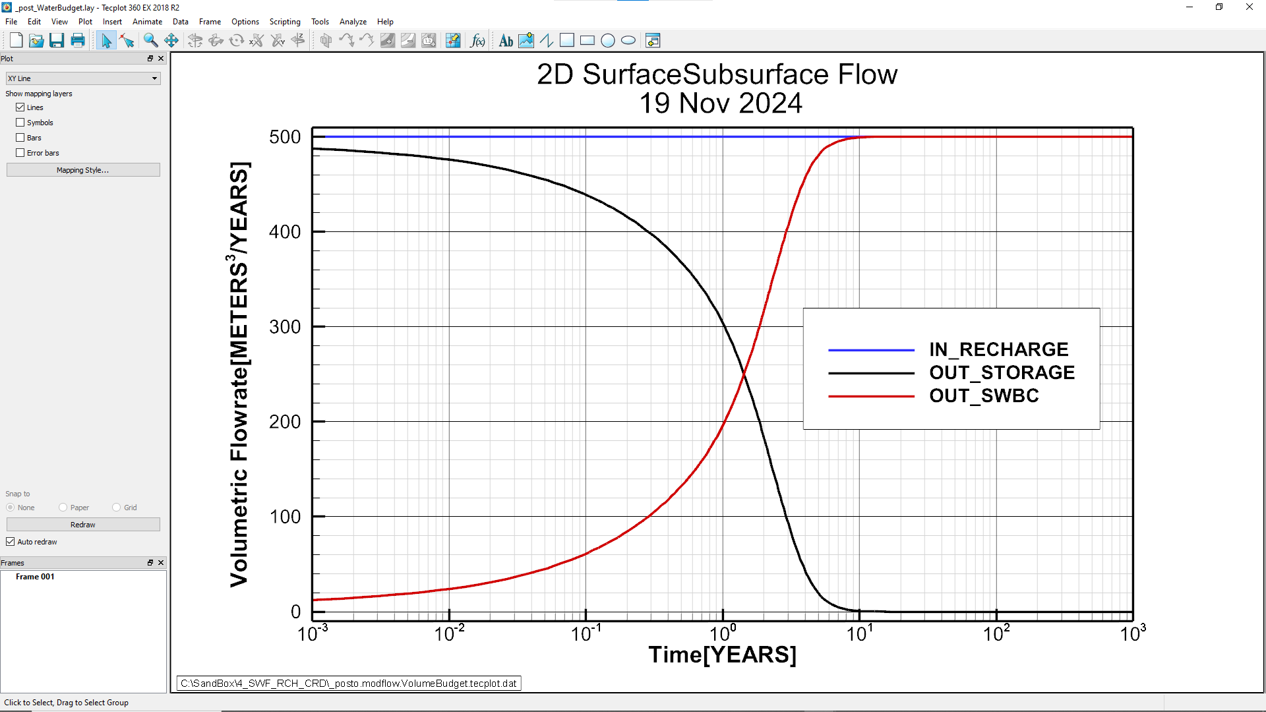
\includegraphics[width=\textwidth]{4_2_Budget}

This \tecplot\ frame has the following features and contents:
\begin{itemize}
  \item It is an {\sf XY Line} plot showing the volumetric flowrate versus time for selected components of the model.
  \item The name of the data file loaded into the frame is shown at the bottom left corner.
  \item The plot title and current date (on the day the file was loaded) are shown centred above the plot.
  \item The line legend is shown on the right side of the plot.
  \item The X-axis uses a log time scale.
\end{itemize}

The \tecplot\ date set information dialogue shows all of the variables available for plotting:

        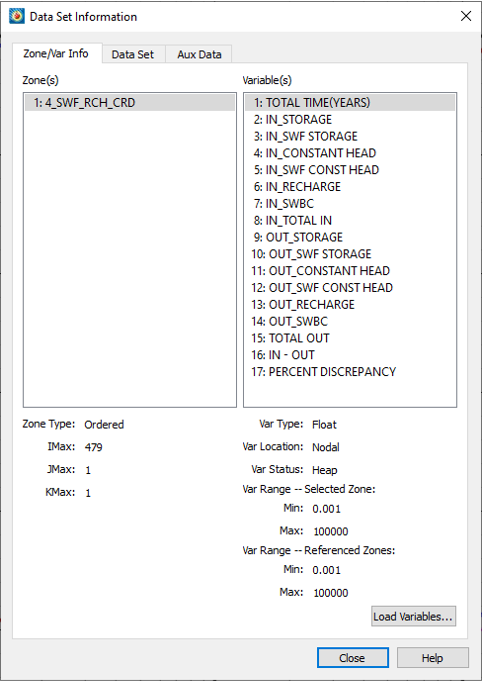
\includegraphics[width=.6\textwidth]{4_3_DataSetInfo}

Variable names are derived from the {\tt modflow.lst} file:
\begin{verbatim}
      VOLUMETRIC BUDGET FOR ENTIRE MODEL AT END OF TIME STEP  479 IN STRESS PERIOD    1
      ----------------------------------------------------------------------------- ---

         CUMULATIVE VOLUMES      L**3       RATES FOR THIS TIME STEP      L**3/T
         ------------------                 ------------------------

               IN:                                      IN:
               ---                                      ---
                 STORAGE =       3.0881E-04               STORAGE =       5.6023E-09
             SWF STORAGE =       9.9743E-03           SWF STORAGE =       2.1841E-13
           CONSTANT HEAD =           0.0000         CONSTANT HEAD =           0.0000
          SWF CONST HEAD =           0.0000        SWF CONST HEAD =           0.0000
                RECHARGE =    50000000.0000              RECHARGE =         500.0000
                    SWBC =           0.0000                  SWBC =           0.0000

                TOTAL IN =    50000000.0103              TOTAL IN =         500.0000

        ... etc

     PERCENT DISCREPANCY =           0.01     PERCENT DISCREPANCY =           0.01
\end{verbatim}


This example has a uniform recharge rate of 0.5 $meters/year$ which results in a total recharge of 500 $meters^{3}/year$ when multiplied by the 1000 $meter$ length of the cross-section. Initially, water comes out of storage then but this declines to zero at equilibrium.  Water exiting the surface water outflow critical depth boundary  {\sf OUT\_SWBC} is initially zero then rises to equal the total recharge at equilibrium.  Fluid balance error {\sf IN-OUT} is essentially zero throughout the simulation.

The probe tool can be used in {\sf XY Line} plots to get exact variable values at a chosen location along the X or Y axis.  The cursor is shown as a vertical line if probing values on the X-axis (i.e.\ over time):

        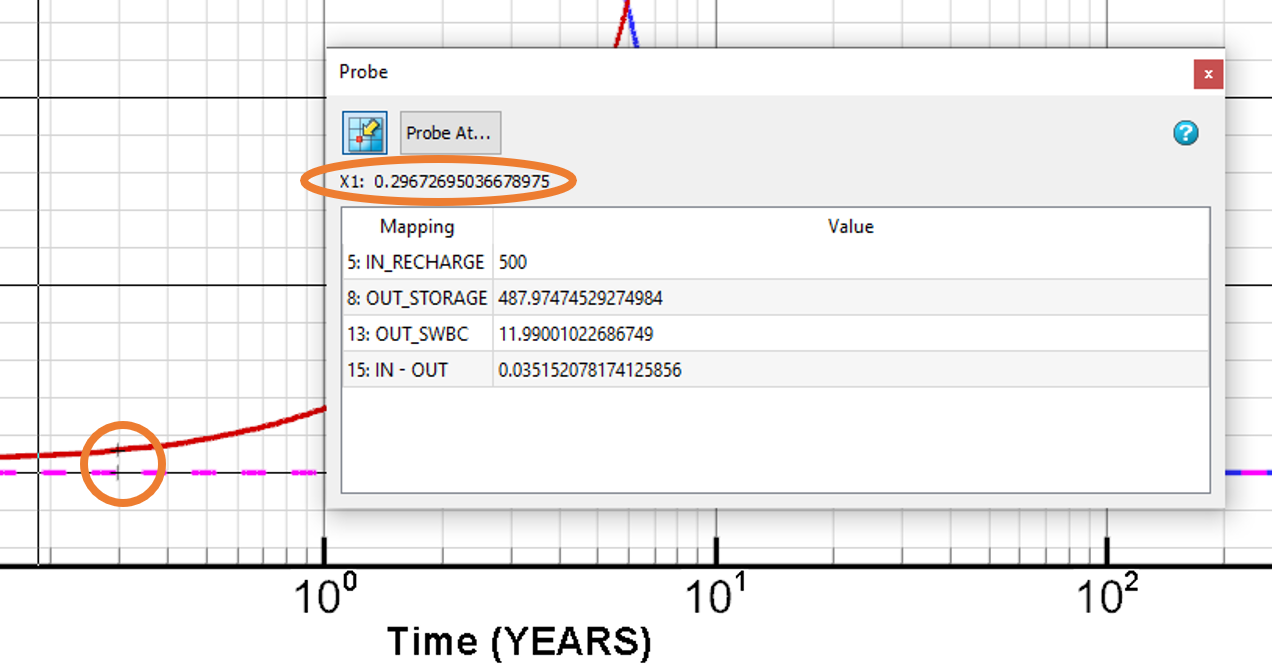
\includegraphics[width=\textwidth]{4_4_Probe}

Here, the location of the probe is shown by small vertical lines placed where the probe crossed the plotted lines (lower left orange circle).  The exact coordinate is given as {\sf X1: 0.2967...}  years.  At this early time, the {\sf OUT\_STORAGE} value is still near its initial value of 500 and the {\sf OUT\_SWBC} has just started rising.

\section{3D Visualization of Model Results}
A \tecplot\ layout file, \texttt{\_post.lay}, has been created for each example and  provides a quick way to view \mfus\ model solution results.  This result is from the example {\tt 6\_Abdul\_Prism\_Cell}:

        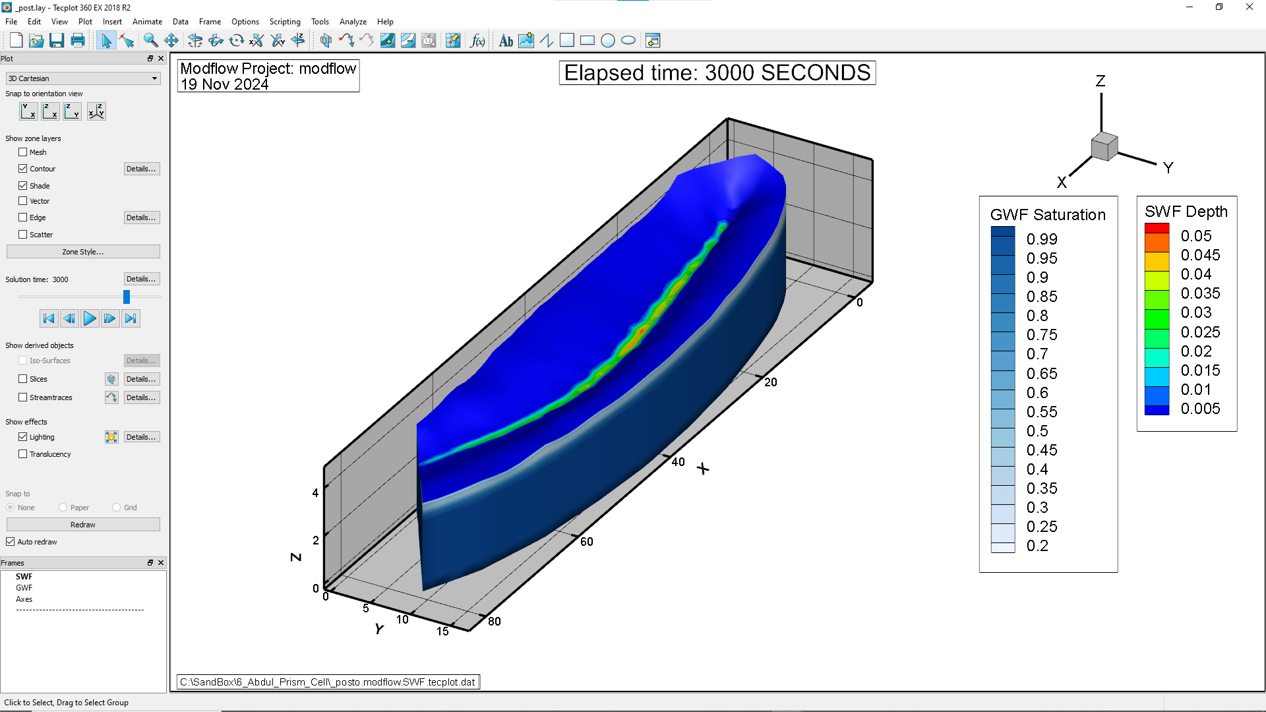
\includegraphics[width=\textwidth]{4_5_Post_Abdul}

The {\tt \_post.lay} layout file is similar to the {\tt \_build.lay} file shown earlier for the same problem: {\sf  SWF, GWF} and {\sf Axes} frames are visible (i.e. placed above the {\sf background} frame in the list).  The {\sf SWF} is currently active (i.e. the name is bolded) and placed at the front of the image (i.e. at the top of the list). It uses a different colormap to make it easier to distinguish the \gwf\ domain below.In this case though, the contoured variables are {\sf SWF Depth} and {\sf GWF Saturation} results from the \mfus\ simulation.

\subsection{Solution Times and Animation}
The model output includes data for several output times, and the image above is showing conditions at a solution time of 3000 seconds, as indicated by the label near the top center of the plot.  The solution time shown is controlled by the slider and button controls near the centre of the {\sf Plot} frame on the left hand side of the image:

        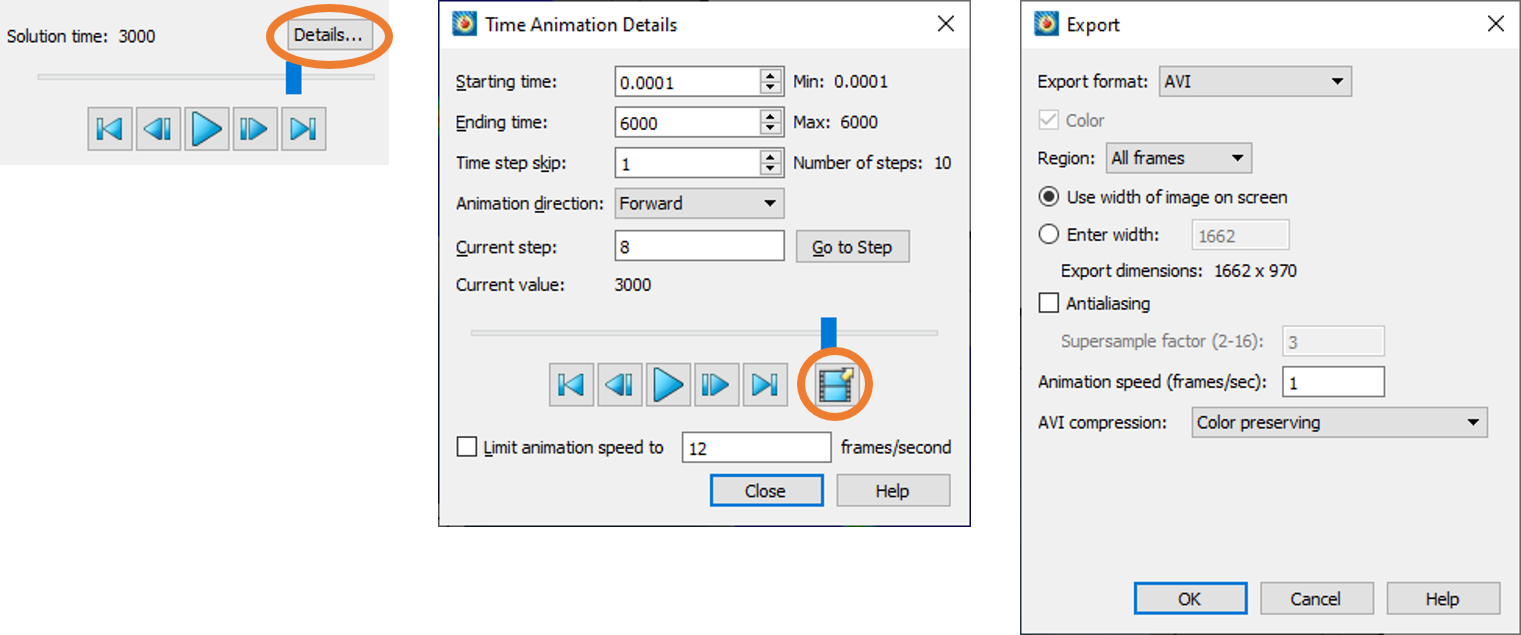
\includegraphics[width=.8\textwidth]{4_6_SolutionSlider}

The {\sf Details...} button leads to the {\sf Time animation details} dialogue which allows you to control and save animations of transient model results using the {\sf Export To File} button 
\includegraphics{ExportToFile}.  There is an example animation in  \texttt{$\backslash$MUT\_Examples-main$\backslash$\-6\_Abdul\_Prism\_Cell} folder in the powerpoint file {\tt Abdul Problem Animation.pptx}.  It used the settings shown in the {\sf Export} dialogue above to limit animation speed and write to an {\tt AVI}-formatted file.  This was then inserted in powerpoint where it can be viewed.

\subsection{Data Set Infomation}
The {\sf Data Set Information} dialogues for the {\sf SWF} and {\sf GWF} frames are shown below:

        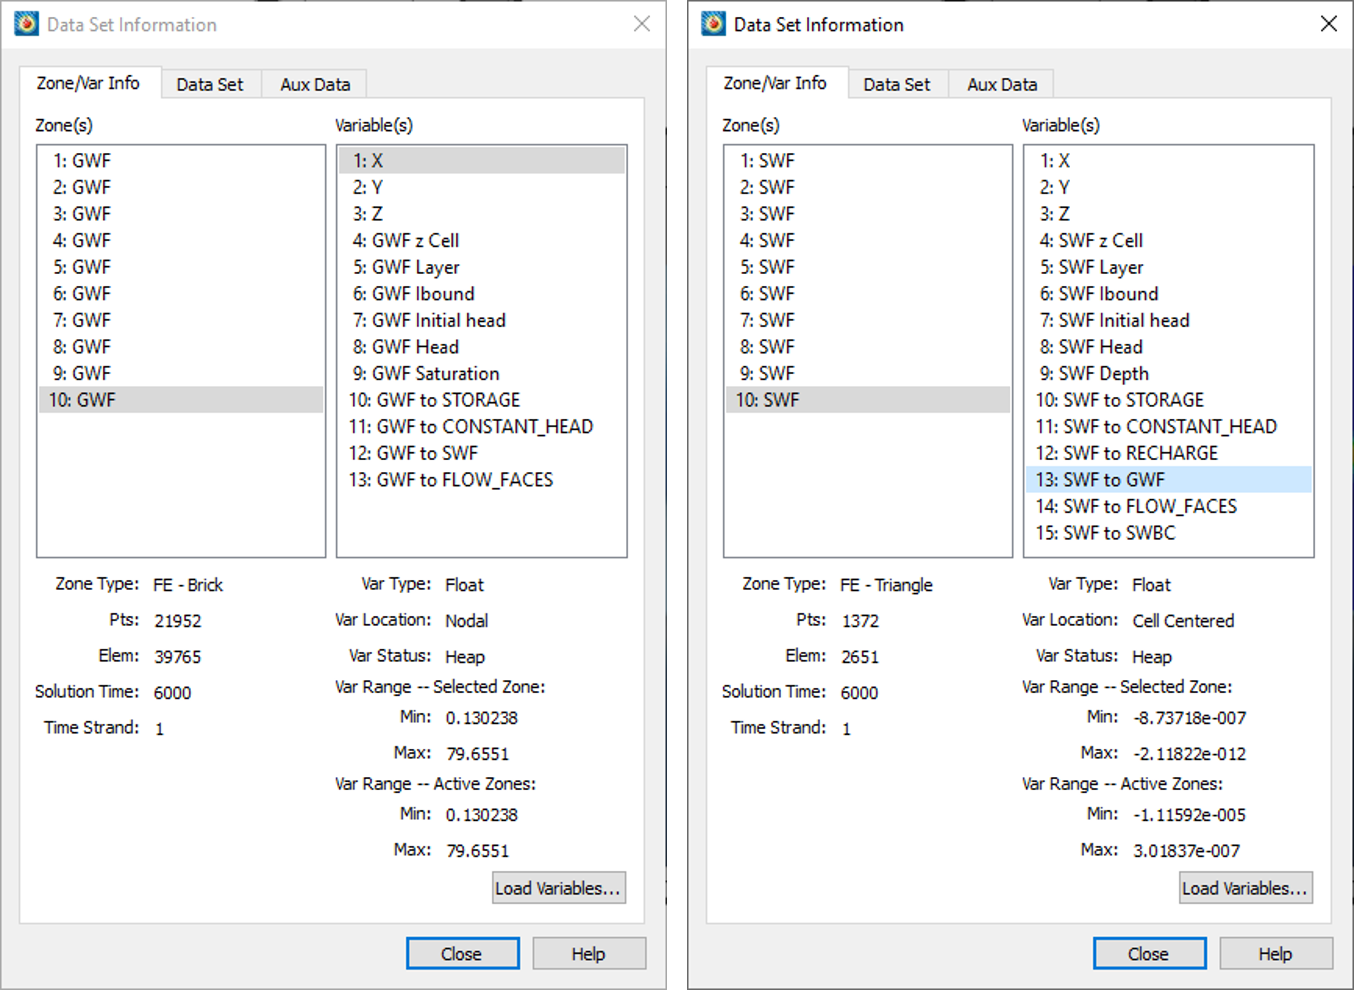
\includegraphics[width=.8\textwidth]{4_7_DatSetInfo}

These are similar to those shown earlier during the model build except there are now multiple {\sf Zone(s)}, one for each output time.  The {\sf Solution Time} (6000) is shown for the highlighted zone, in this case zone 10.

Included are these cell properties:
\begin{itemize}
    \item Elevation {\sf SWF z Cell} and {\sf GWF z Cell}.
    \item \mf\ layer number  {\sf SWF layer} and {\sf GWF layer}.
    \item \mf\ boundary number {\sf SWF Ibound} and {\sf GWF Ibound}.
    \item Initial head.
    \item Hydraulic head result.
    \item \gwf\ saturation and \swf\ depth.  These are stored in the \mf\ DDN (drawdown) file.
    \item In this case, cell-by-cell flows are stored in \gwf\ variables 10 to 13 and \swf\ variables 10 to 15.
\end{itemize}

\subsection{Inactive Cells and Value Blanking }
The example {\tt 6\_Abdul\_MODHMS} was generated from a 2D rectangular template mesh.  To make it conform to the shape of the original triangular mesh used in example  {\tt 6\_Abdul\_Prism\_Cell}, a region of inactive cells was assigned around the outside of the domain.  The layout file {\sf \_plot.lay} has been configured to show only active cells:

        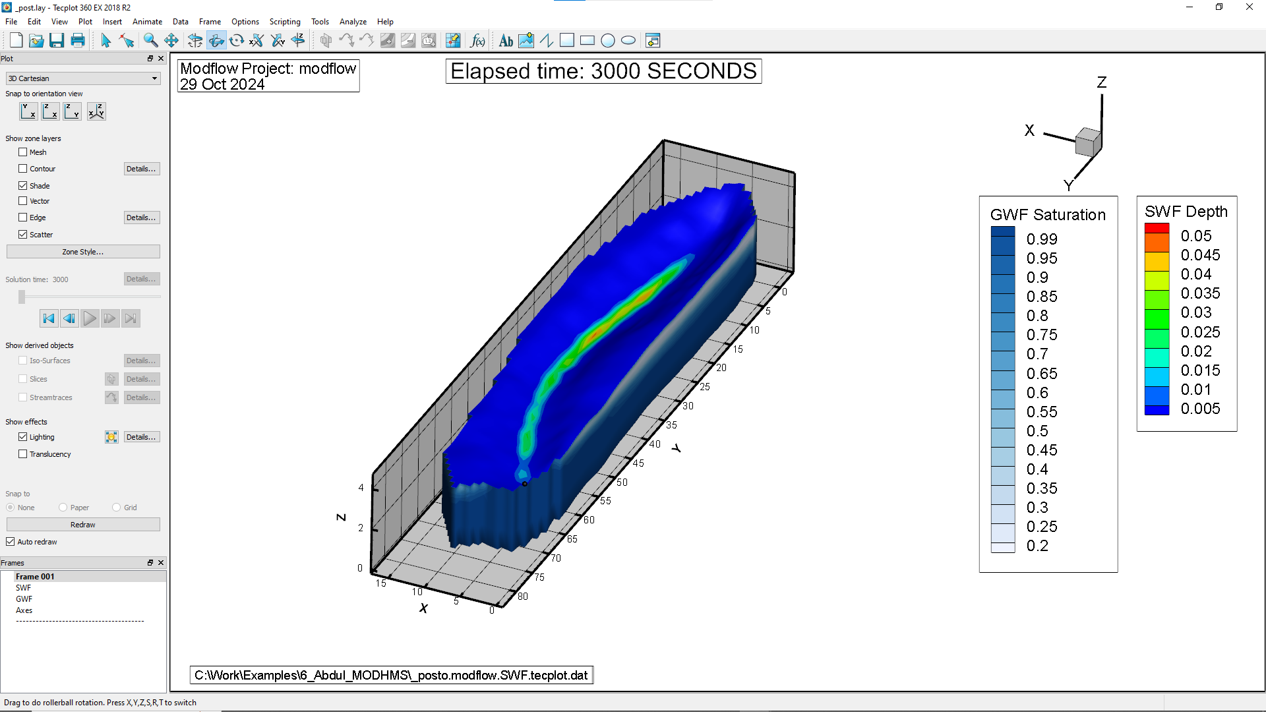
\includegraphics[width=.8\textwidth]{4_7a_MODHMS}

 The layout uses \tecplot\ value-blanking \index{\tecplot\ ! value blanking} (in this case based on the value of the blanking variables {\sf SWF Ibound} and {\sf GWF Ibound}) to prevent cells (or portions of cells) from appearing in the image.  The {\sf Plot$\backslash$Blanking$\backslash$Value Blanking...} menu option leads to the {\sf Value Blanking} dialogue for the currently active frame:

        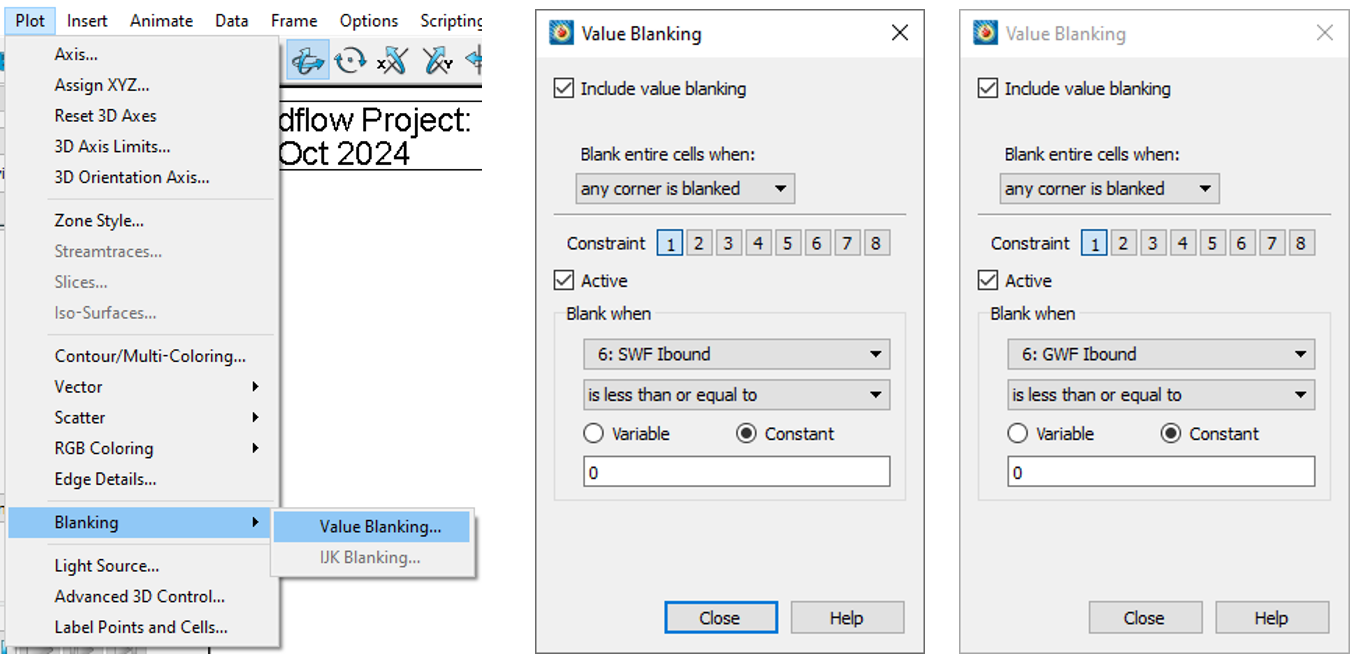
\includegraphics[width=.8\textwidth]{4_7b_ValueBlanking}

Shown here are the dialogues for both the \swf\ and \gwf\ domains, where value blanking constraints are set to prevent \swf\ and \gwf\ domain cells from being shown if the {\sf SWF Ibound} or {\sf GWF Ibound} value is less than or equal to zero.

\subsection{Slices and Fence Diagrams}
The layout file {\tt 6\_Abdul\_Prism\_Cell$\backslash$\_GWF\_Saturation\_Slices.lay} has been configured to show a series of cross-sections in the \gwf\ domain:\index{\tecplot\ ! Slices and Fence diagrams}

        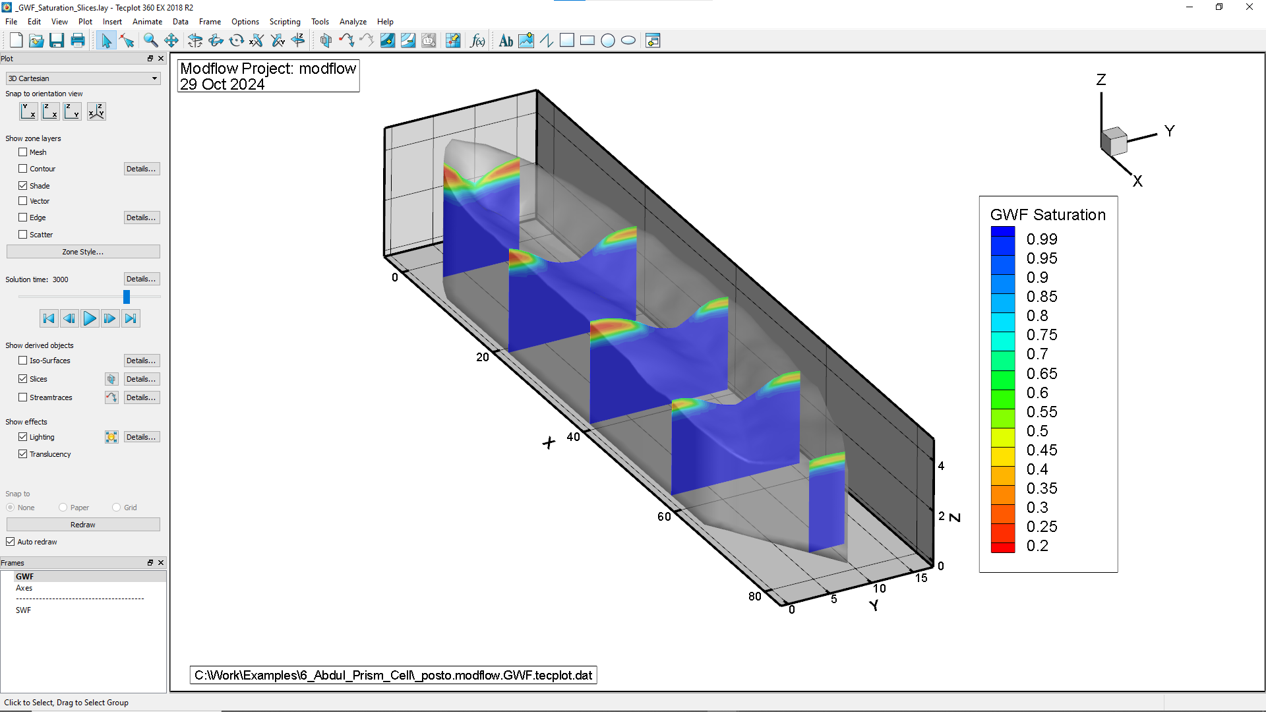
\includegraphics[width=.8\textwidth]{4_8_Slices}

The layout uses the \tecplot\ derived object {\sf Slices} to define the slice locations and content. The {\sf Details...} button leads to the {\sf Slice Details} dialogue for the currently active frame:

        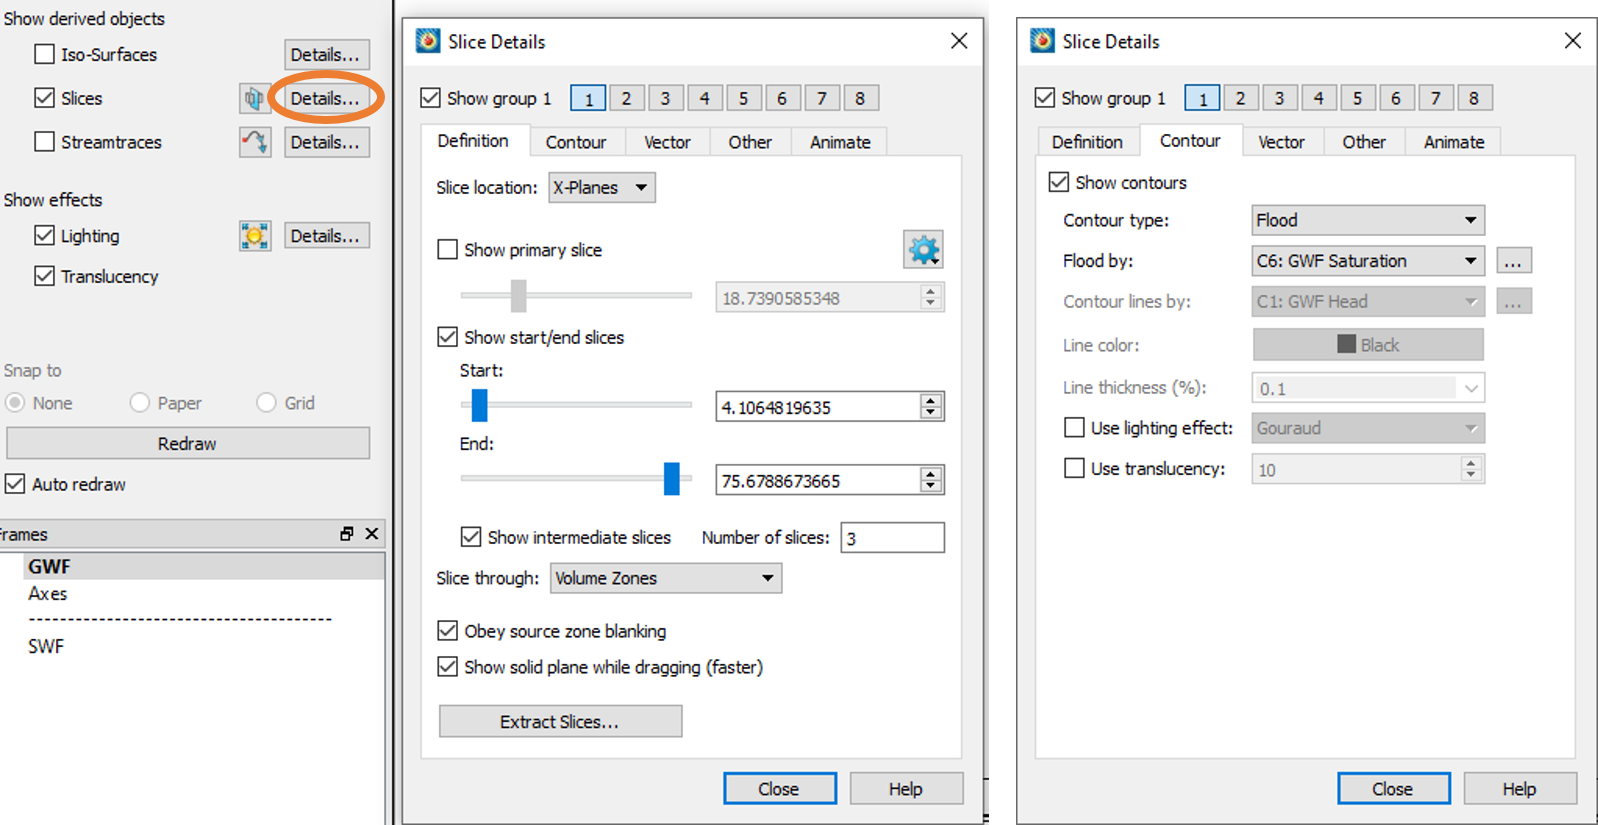
\includegraphics[width=.8\textwidth]{4_9_SliceDetails}

The {\sf Definition} tab is configured to position the start and end slice positions and set the number of intermediate slices at 3.

The {\sf Contour} tab is configured to contour-flood the slices by {\sf GWF Saturation} value.

The {\sf Shade} and {\sf Translucency} boxes are checked to show the slice position relative to the model domain.

\subsection{Defining New Variables}
\index{\tecplot\ ! Equations and defining new variables}
New variables can be defined in \tecplot\ using the {\sf Data$\backslash$Alter$\backslash$Specify equations...} menu option which leads to the {\sf Specify equations} dialogue:

        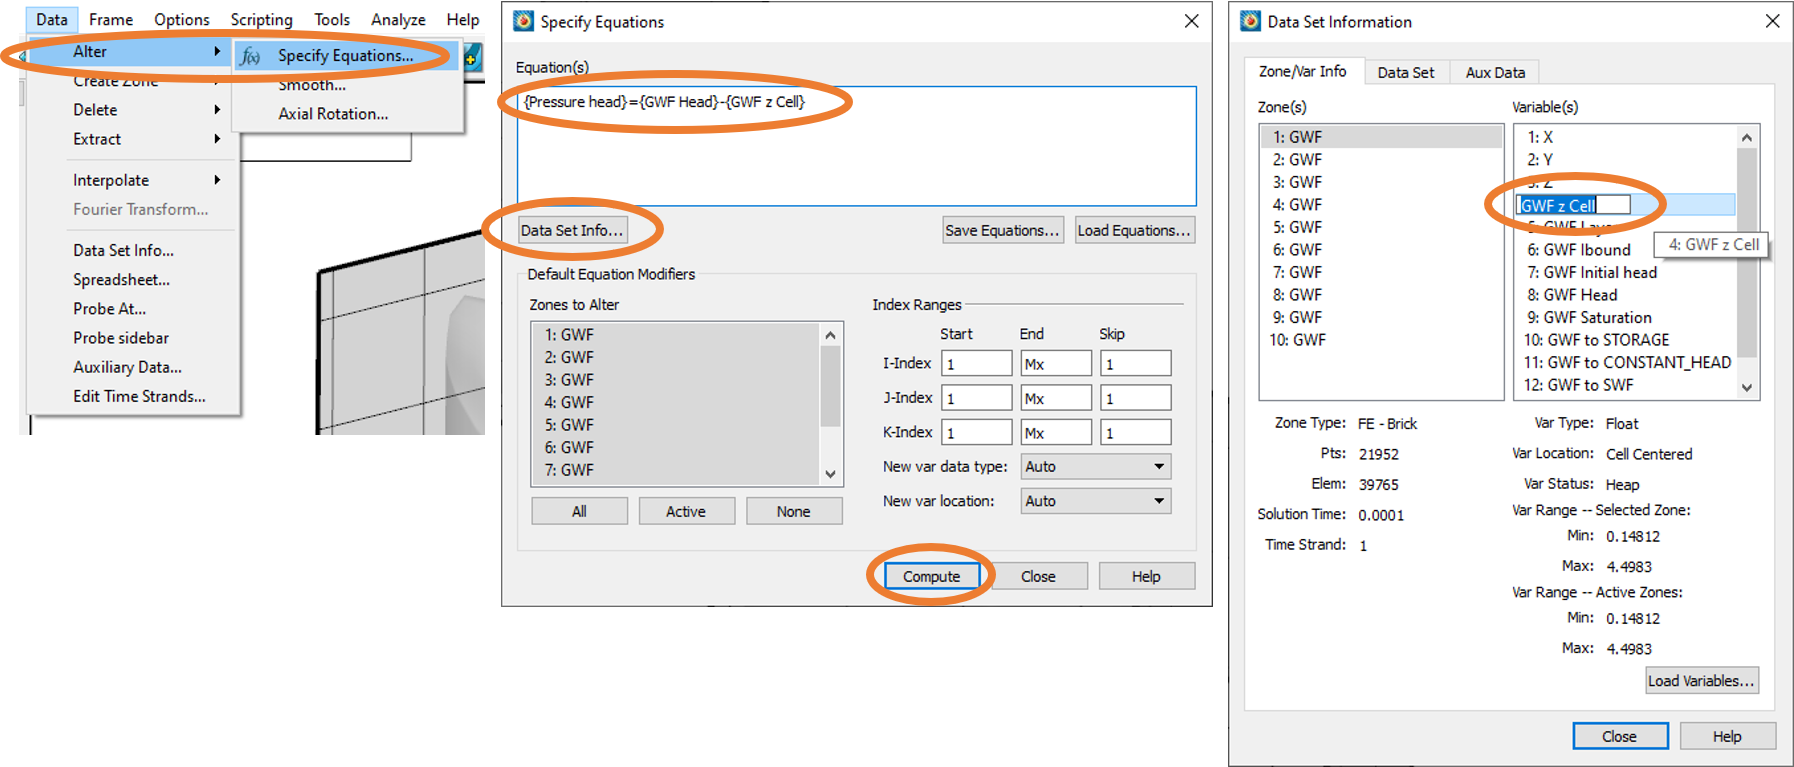
\includegraphics[width=.8\textwidth]{4_10_Equations}

This dialogue has an {\sf Equation(s)} window where we have defined a new variable, in this case {\sf Pressure Head},  that is calculated from two existing variables according to the  mathematical expression: 

{\sf \{Pressure Head\} = \{GWF Head\}  -\{GWF z Cell\}}  

In equation syntax, variable names must be placed within curly brackets: {\sf \{\}}.

The {\sf Data Set Info...} tab leads to the {\sf Data Set Information} dialogue where variable names can be cut and pasted into the equation window.  Here the {\sf GWF z Cell} variable has been selected.

Once the equation is complete, click the {\sf Compute} button to generate the new variable, which will now show up in the {\sf Data Set Information} dialogue:

        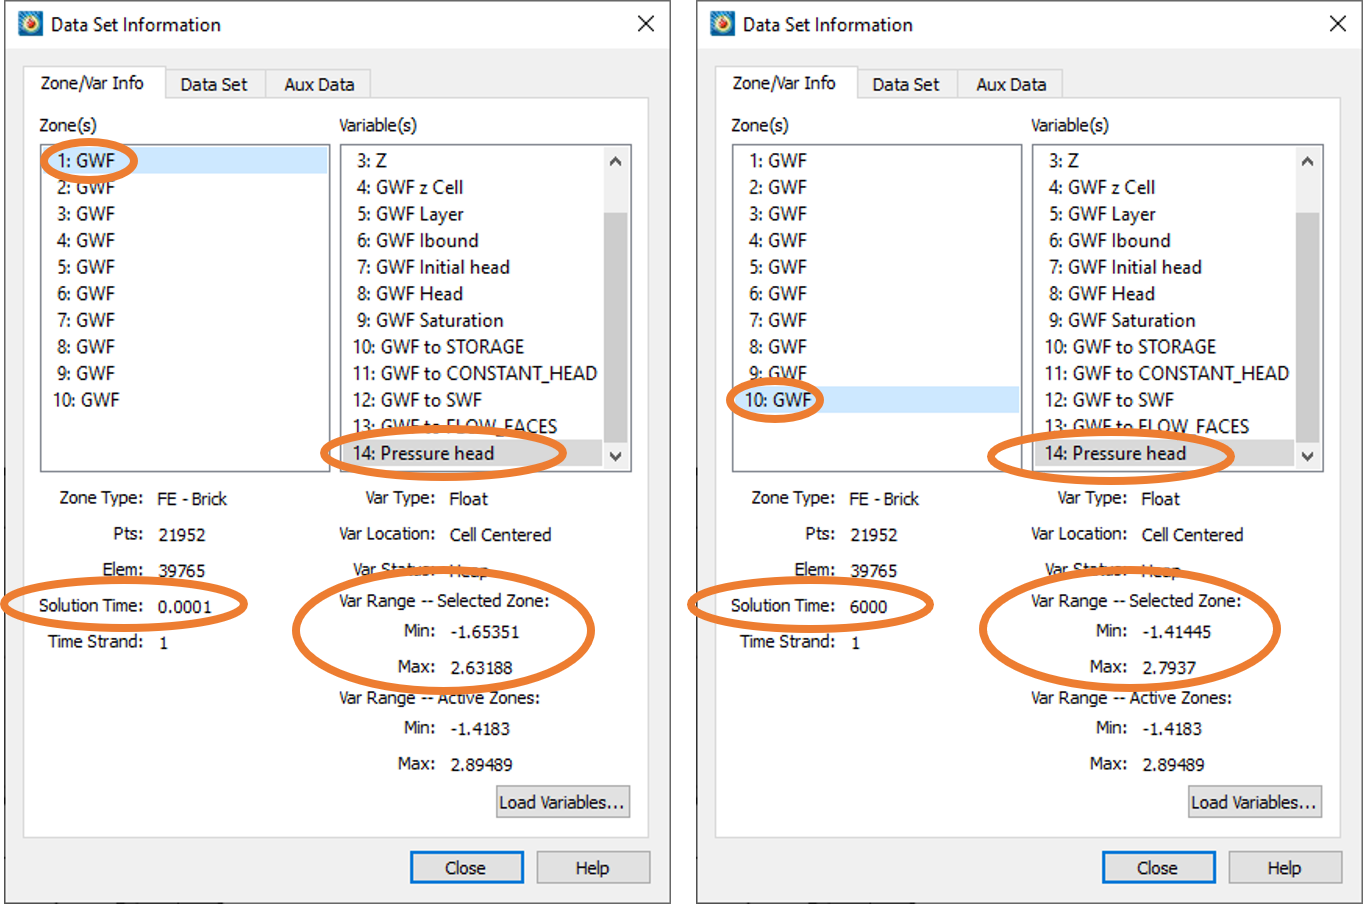
\includegraphics[width=.8\textwidth]{4_11_PressureHead}

Here we see the variable {\sf 14:Pressure Head} has been added. Because the {\sf GWF Head} variable changes over time and is defined at every timestep, the calculated variable does also.  The two panes above show the pressure head range at solution time 0.0001 is different at time 6000.

\mfus\ uses the \mf\ {\it DDN} (i.e. drawdown) file to store saturation values for the \gwf\ domain and surface water depth values for the \swf\ domain. If you want to plot drawdowns they can be calculated by adding an equation to the previous example:

        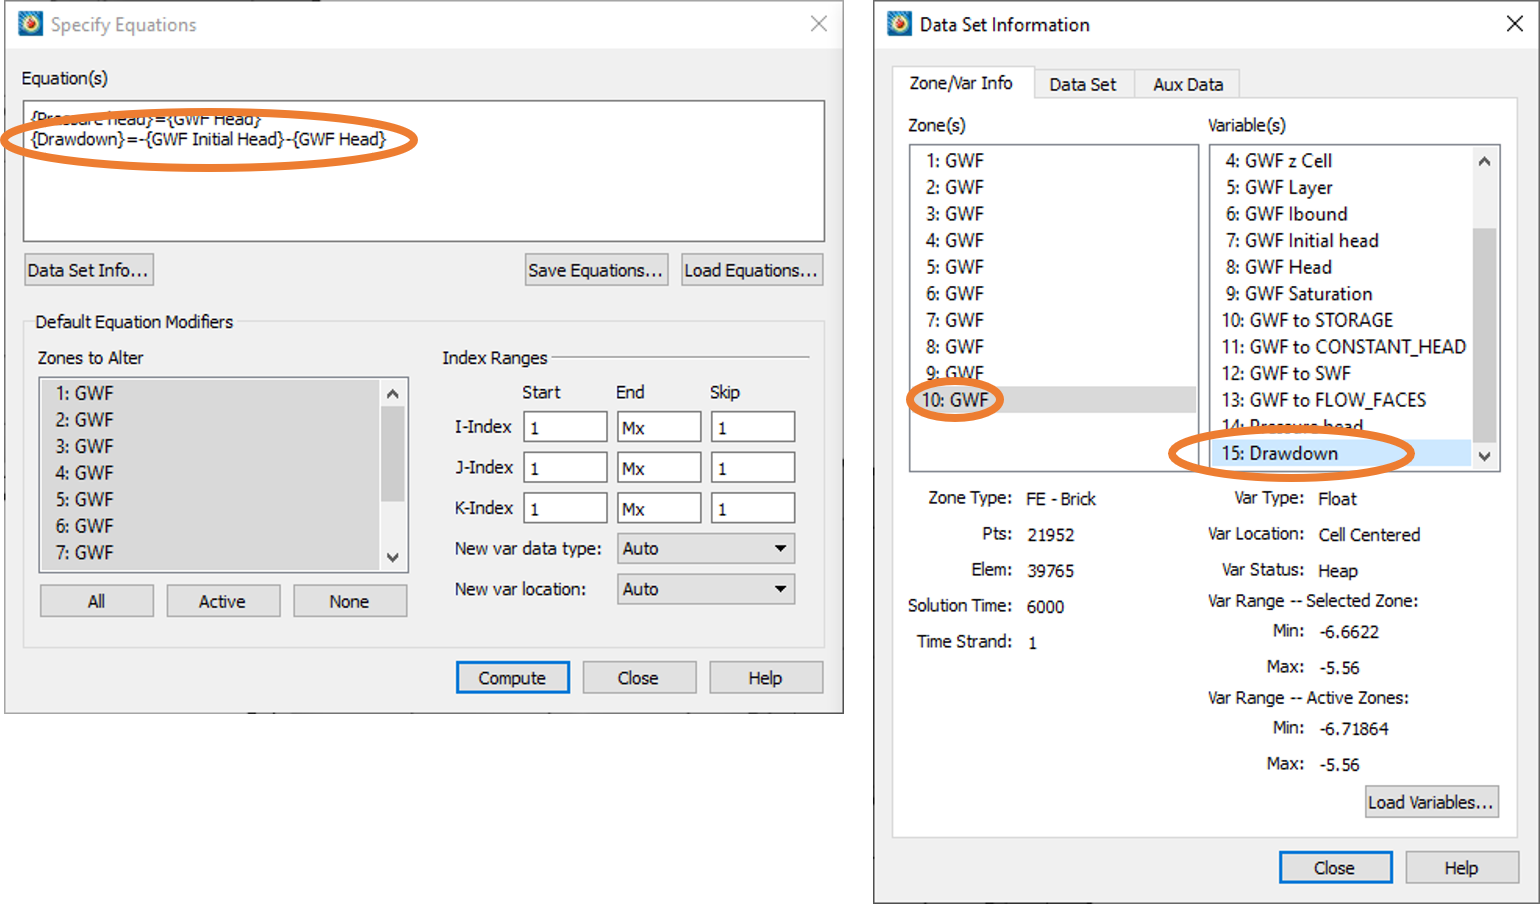
\includegraphics[width=.8\textwidth]{4_12_Drawdown}

Here we see the equation for calculating the variable {\sf Drawdown} has been added to the {\sf Equations(s)} window and the variable {\sf 15:Drawdown} appear in the {\sf Data Set Information} dialogue.  The range shown for {\sf Drawdown} values is negative because simulated heads were always higher than the initial flat water table condition.

\subsection{Water Table Isosurface Plot}
\index{\tecplot\ ! Isosurfaces, Water Table Plot}
The layout file {\tt 6\_Abdul\_Prism\_Cell$\backslash$\_Water\_Table.lay} has been configured to show an isosurface of the water table in the \gwf\ domain at a time of 3000 seconds :\index{\tecplot\ ! Slices and Fence diagrams}

        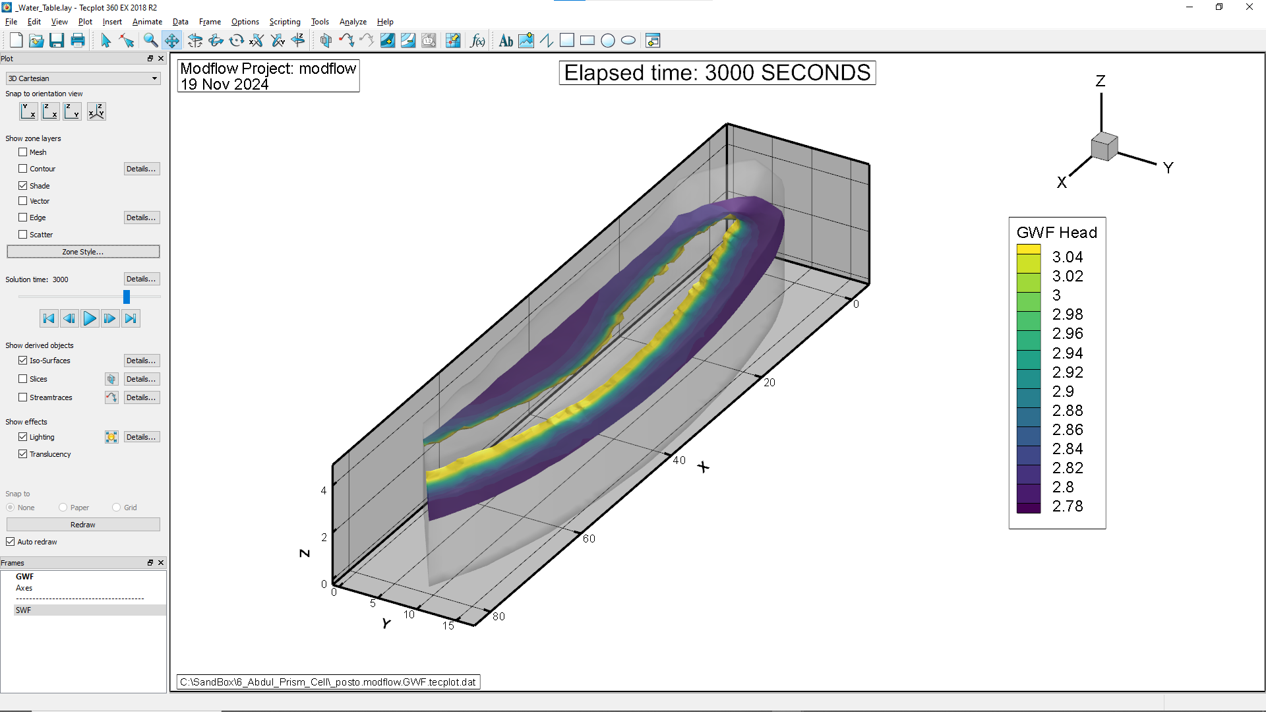
\includegraphics[width=.8\textwidth]{4_13_Isosurface.png}

The layout uses the \tecplot\ derived object {\sf Iso-surfaces} to define the slice locations and content. The {\sf Details...} button leads to the {\sf Iso-Surface Details} dialogue for the currently active \gwf\ frame:

        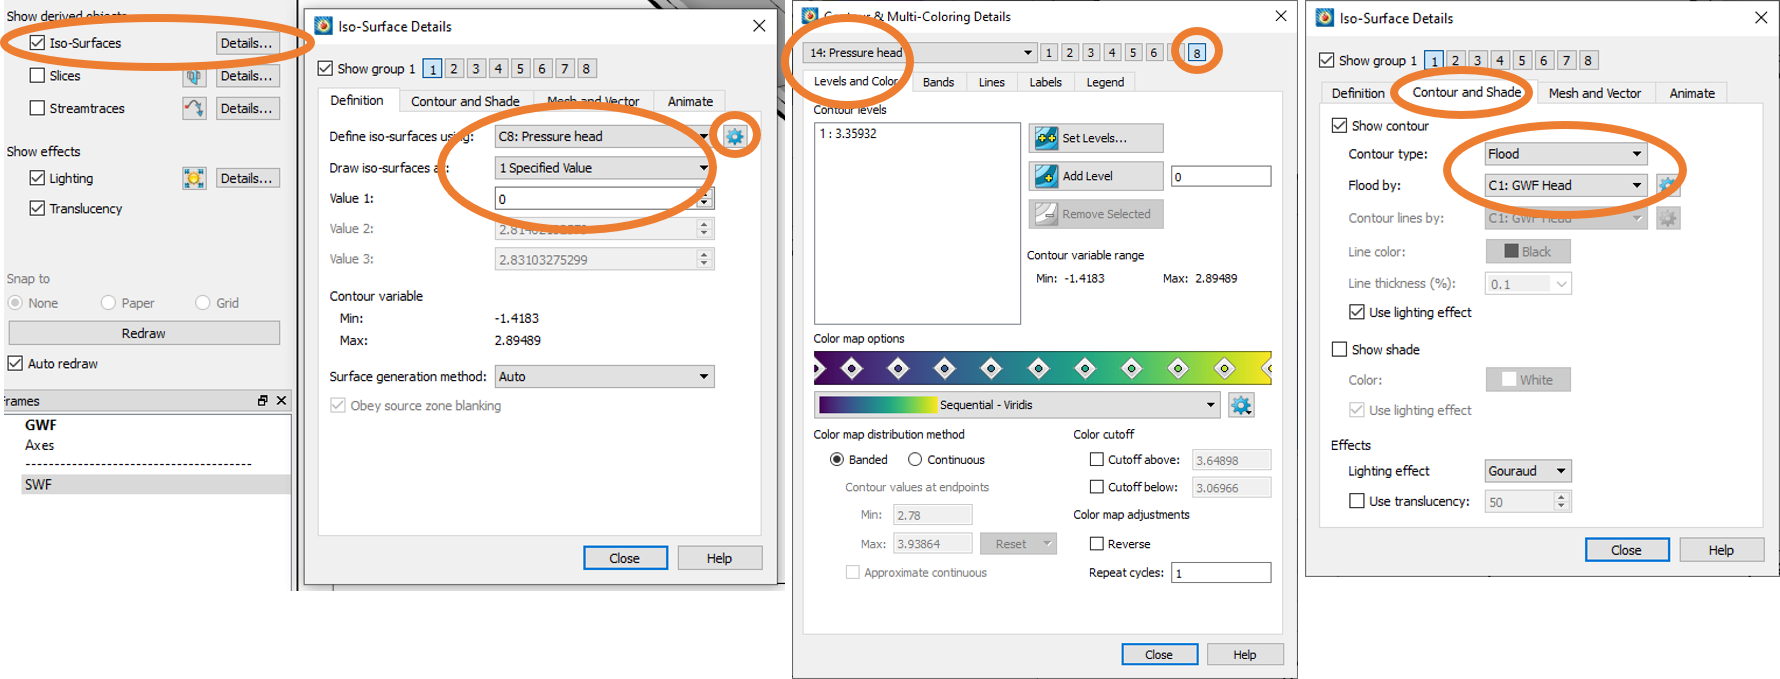
\includegraphics[width=\textwidth]{4_15_IsosurfaceDetails}

The {\sf Definition} tab is configured to define iso-surfaces using the {\sf Pressure Head} variable. This had to be defined as one of the eight contouring variables, and there is a short-cut to the {\sf Contour \& Multi-Colouring Details} dialogue using the 
\includegraphics{GearButton} button, where we set the eighth contouring variable (number 8 in orange circle) as {\sf 14:Pressure Head}.  By definition, the water table is the surface where the pressure head is equal to zero, so back on the {\sf Definitions} tab we chose to draw iso-surfaces at one specified value: zero.

Finally, the {\sf Contours and shade} tab is configured to contour flood the isosurface with the {\sf GWF Head} variable.

\subsection{Infiltration Plot}
\index{\tecplot\ ! Infiltration Plot}
The layout file {\tt 6\_Abdul\_Prism\_Cell$\backslash$\_Infiltration} defines a new variable {\sf Infiltration [mm/hour]} and uses contour flood and lines to show it.  The contour levels are set up with a red-blue colour map that is symmetric about the value zero. Red shading indicates zones of infiltration, while blue shading indicates zones of \gwf\ discharge to the \swf\ domain.

        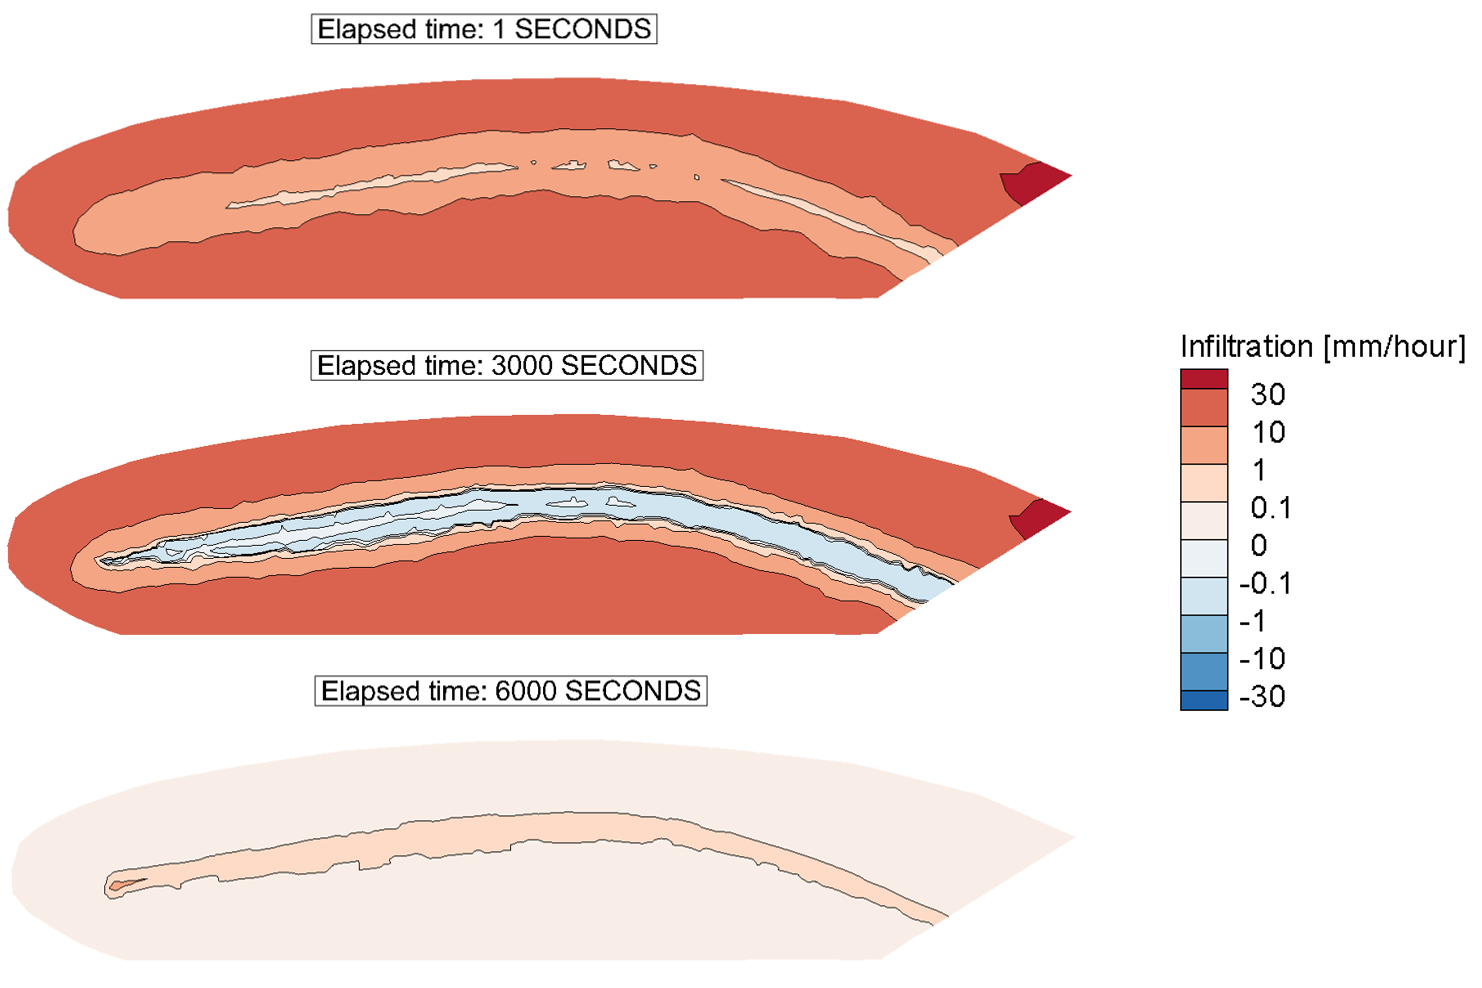
\includegraphics[width=\textwidth]{4_16_Infiltration.png}

Here we can see the infiltration at 3 times:
\begin{description}
\item [1 second] The application of water to the \swf\ domain has just started.  The entire \swf\ domain is shaded red, showing that water is infiltrating everywhere, with the highest rate of infiltration occurring at the highest elevations in the domain (i.e.\ at hilltops)
\item [3000 seconds] Application of water stops.  Infiltration is still occurring on the hills but discharge is occurring along most of the length of the swale, as shown by the blue shaded region.
\item [6000 seconds] End of simulation.  The stream has drained and water is again infiltrating over the entire  domain.
\end{description}

The new  variable {\sf Infiltration [mm/hour]} is calculated by the following equation in \tecplot:

        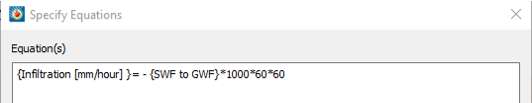
\includegraphics[width=.8\textwidth]{4_17_Infiltration_eqn}

The variable {\sf SFW to GWF} contains the cell-by-cell flows from the \swf\ domain to the \gwf\ domain, with negative values indicating a loss relative to the \swf\ domain (i.e.\ infiltration).  We want infiltration to be shown as a positive value in this case so we add a negative sign at the beginning of the equation.  The final part of the equation {\sf *1000*60*60} converts the value from units of meters per second to millimetres per hour.

The contour levels were set up as shown here:

        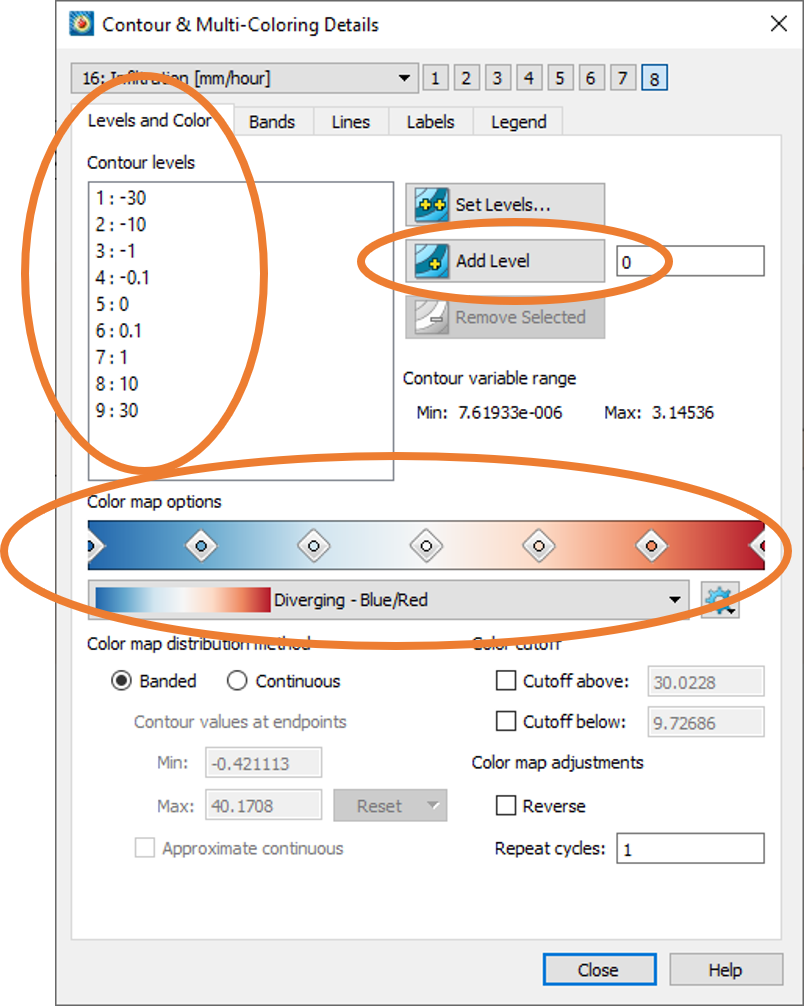
\includegraphics[width=.6\textwidth]{4_18_Infiltration_contour}

The levels were entered manually using the {\sf Add Level} and {\sf Remove selected} buttons.  The value zero is defined at the boundary between blue and red colours by using an equal number of positive and negative values with the same absolute ranges.

The color map is set to {\sf Diverging - Blue/Red} using the drop-down menu.


